\documentclass[10pt]{article}
\usepackage[margin=0.65in]{geometry}
\usepackage{graphicx,mathptmx}
\usepackage[hidelinks]{hyperref}
\title{Checked hash-prime setup for native ECCp-131}
\author{Engineering and bounded correctness receipt}
\date{30 October 2026}
\begin{document}
\maketitle
\noindent The curve already accepts checked p/r proofs. This follow-up retains
verified auxiliary prime facts for hash-modulus setup, factor bases and replay.
The source permits a fixed prime $s\in[2p,4p]$; uniform hash seeds are preserved.
An optional declared modulus enables this path. Default random selection keeps
its candidate stream and RNG draws. Uncovered values retain exact primality.
\begin{center}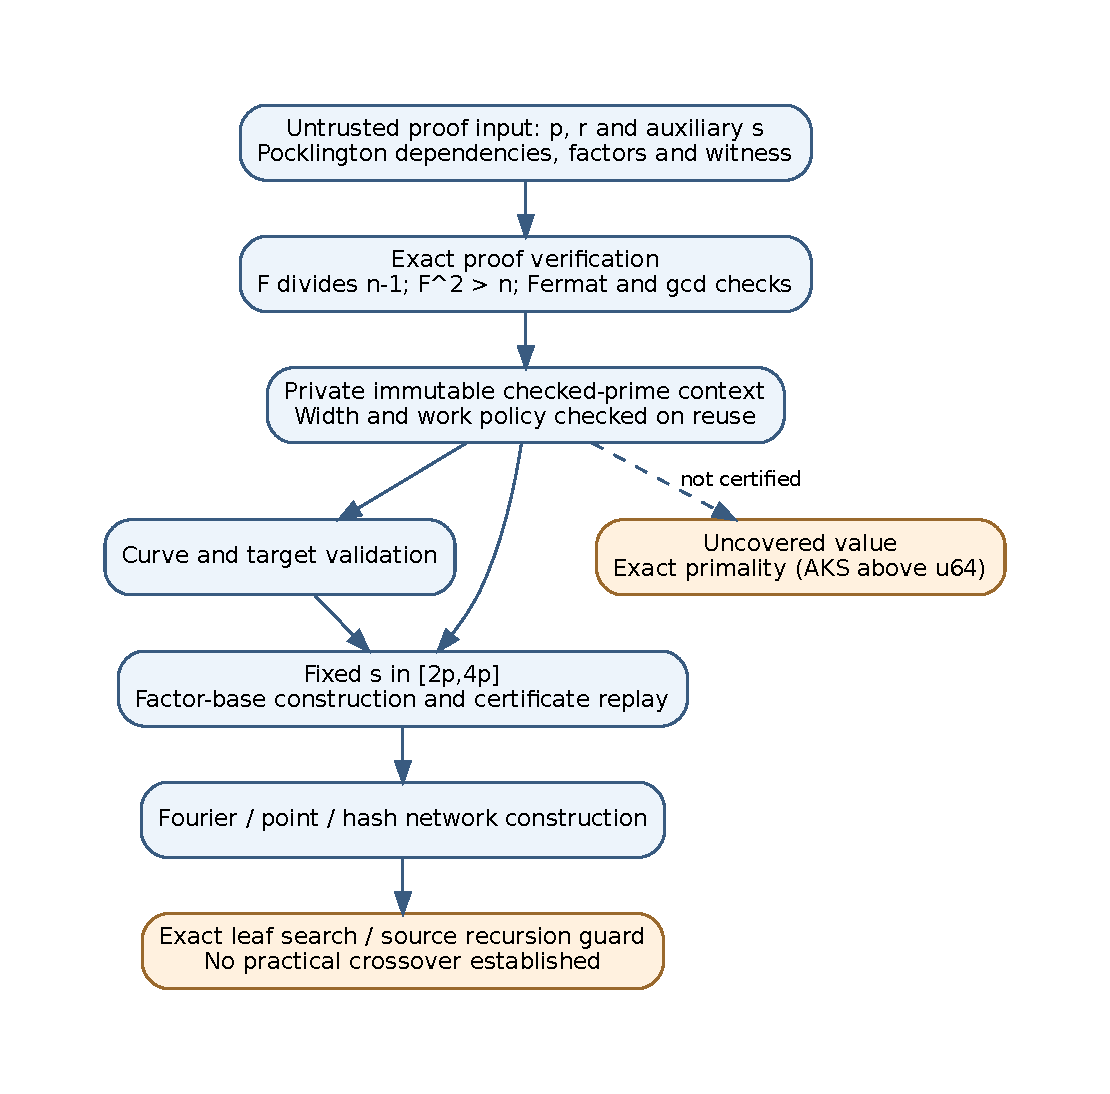
\includegraphics[width=0.9\linewidth,height=3.7in,keepaspectratio]{setup.pdf}\end{center}
\noindent\textbf{Development evidence.} Six targeted controls pass, including a
65-bit proof, official 132-bit hash modulus, resource limits, missing proof,
tiny known-answer solve/replay and runner pin rejection. Official parameter,
target and hash preflight charges 5,897 uncalibrated steps under the original
two-million-step policy. Fixture preparation checks 68 candidate proofs and
charges 371,334 diagnostic steps. These are not timing measurements; proof
generation belongs in future cold accounting. No runtime gain is established.

\smallskip\noindent\textbf{Limits.} The unchanged literal recursion guard requires
$E>2^{131070}$ before its root scale can become positive; additional guards also
apply. Machine-sized graph indices keep this production scale zero. Generic
uncertified large-prime setup, practical search, both challenge solves and the
independent full audit remain open. No profile or scientific benchmark ran.
The user's Fourier-construction timings are attributed observations, not
independently admitted results here; primality hangs do not show construction
infeasibility. S3 checkpoint upload/readback has succeeded separately.

\smallskip\noindent\textbf{Sources and evidence.}
\href{https://github.com/bochum-crypto/subexponential-ecdl/tree/1ee44e562b1b9a50ea339f3b8f81112b5a24b96f}{Bochum v0.2, section 3};
\href{https://cacr.uwaterloo.ca/hac/about/chap4.pdf}{HAC Fact 4.40};
the existing native source guards, new checked JSON fixture and retained
development transcripts/source manifests beside README.md. Existing frozen
reports, theorem constants, curves and leaderboard evidence are unchanged.
\end{document}
